\documentclass{cumcmthesis}
%\documentclass[withoutpreface,bwprint]{cumcmthesis} %去掉封面与编号页。

%声明:本模板基于CUMCMThesis项目修改而来,适用于全国大学生信息安全竞赛作品赛
%仅供学习交流使用,侵删
%author:ShenaoW from XDU SCE
%cooperator:PoliScope项目组
%email:shenaowang@foxmail.com
%date:2022.05.24

\usepackage[framemethod=TikZ]{mdframed}
\usepackage{url}   % 网页链接
\usepackage{subcaption} % 子标题
\usepackage{colortbl}
\usepackage{color}
\definecolor{tabcolor}{RGB}{42, 110, 63} % 这里就是我们怎么定义我们的表格的线宽颜色
% 伪代码
\usepackage[noend]{algpseudocode}
\usepackage{algorithmicx,algorithm}
% 页眉页脚
\usepackage{lastpage}
\usepackage{fancyhdr} % 导入fancyhdr包
\pagestyle{fancy}
% 图表、公式按章节编号
\usepackage{amsmath}
\numberwithin{equation}{section} % 公式按章节编号
\numberwithin{figure}{section} % 图按章节编号
\numberwithin{table}{section} % 表按章节编号



% 设置封面页内容
\titlename{基于DID身份的医疗系统}
\email{22373561\_hyz@buaa.edu.cn}
\yearinput{2024}
\monthinput{05}
\dayinput{24}

% 页眉设置
\fancyhead[L]{}
\fancyhead[R]{}
\fancyhead[C]{\zihao{-5} 基于 DID 身份的医疗系统}
% 页脚设置
%\fancyfoot[L]{左页脚}
\fancyfoot[C]{\zihao{-5} 第\thepage 页 \enspace 共 \pageref{LastPage} 页} % 页码
%\fancyfoot[R]{右页脚}
\renewcommand{\headrulewidth}{0.5pt} % 页眉分隔线宽度0.5磅
%\renewcommand{\footrulewidth}{0.5pt}  % 页脚分隔线宽度0.5磅

\begin{document}
	
% 将\usepackage{ulem}宏包中的\emph{}还原为斜体
\normalem

% 生成封面页和填写说明页	
\maketitle
 
% 生成目录
\newpage
\thispagestyle{empty}
\tableofcontents
\newpage
 
%% 生成图目录
%\thispagestyle{empty}
%\listoffigures
%\newpage
%
%% 生成表目录
%\thispagestyle{empty}
%\listoftables
%\newpage

% 从此处开始编页
\setcounter{page}{1}
 
%中文摘要
\begin{cnabstract}
	
(请简要说明创作本作品之动机、功能、特性、创新处、实用性)

在当今数字化时代,随着信息技术的迅猛发展,患者就诊时医疗数据的产生和积累呈指数级增长,涵盖了个人诊疗状况、疾病诊断信息和基因组数据等,这些数据在就诊时的及时传递与共享对于患者的治疗决策、疾病确诊、临床治疗等方面具有重要意义。

然而,医疗数据的安全共享和利用同样面临着极大的挑战。一方面,现有的医疗机构存储的医疗数据往往仅在内部管理共享,彼此间并不相通,造成严重数据孤岛现象,使患者在进行跨机构就诊时需要准备多份电子病历;另一方面,医疗数据中包含患者的个人隐私敏感信息,在内部共享环境下仍存在部分医疗机构内部人员在未经患者同意的情况下使用这些数据,可能会导致患者隐私泄露;此外,医疗数据还具有一定的商业价值,如利用这些数据来定向投送医疗广告等,很容易成为不法分子恶意攻击进行牟利的对象。因此,在实现医疗数据多机构共享平台的同时,能够保障个人隐私安全具有重要的现实意义。

针对这些问题,基于分布式身份(Decentralized Identifiers,DID)技术实现医疗数据传递共享的想法应运而生。DID技术基于区块链和分布式账本等技术,具有区块链透明、可追溯、不可篡改等优良特性,为每个参与者提供了独一无二的身份标识,实现了去中心化、安全、可验证的身份认证和授权管理。

通过基于DID技术的医疗数据共享方式,医疗数据的共享变得更加安全、高效和透明。医疗机构、医生、患者和研究人员可以在平台上自主管理和控制自己的数据,通过扫码等方式授权合适的权限给其他参与者,实现了医疗数据的可信共享和跨组织的协同合作。此外,基于智能合约的数据访问控制机制结合加密技术可以确保数据的安全性和隐私保护,有效解决了医疗数据共享中的信任和隐私问题。

在这样一个背景下,本文将设计与实现一种基于DID技术的医疗数据交换平台,分析其在促进医疗数据共享、优化医疗资源配置、保障隐私安全等方面的作用和价值,为医疗行业的数字化和个人隐私的安全保护提供支持。

(还会调整)
	
\cnkeywords{1 \quad 2 \quad 3 \quad 4}
\end{cnabstract}

%英文摘要
\begin{enabstract}


\enkeywords{Privacy Compliance \quad NER \quad Static Analysis \quad Dynamic Analysis}
\end{enabstract}

\section{作品概述}

\subsection{背景分析}

随数字化时代的迅猛发展,新兴信息技术为现代化数字医疗系统带来了更多可能。与此同时,医疗健康数据的种类与规模也快速增长,涵盖了患者个人诊疗状况、疾病诊断信息和基因组数据等,这些数据的及时传递与共享对于患者的治疗决策、疾病确诊、临床治疗等方面具有重要意义。

然而,医疗数据的安全共享和利用同样面临着极大的挑战。一方面,现有的医疗机构存储的医疗数据往往仅在内部管理共享,彼此间并不相通,造成严重数据孤岛现象,使患者在进行跨机构就诊时需要准备多份电子病历;另一方面,医疗数据中包含患者的个人隐私敏感信息,在内部共享环境下仍存在部分医疗机构内部人员在未经患者同意的情况下使用这些数据,可能会导致患者隐私泄露;此外,医疗数据还具有一定的商业价值,如利用这些数据来定向投送医疗广告等,很容易成为不法分子恶意攻击进行牟利的对象。可见,在实现医疗数据快速共享的同时,如何保障个人隐私安全成为了医疗行业数字化的一大难题。

\subsection{相关工作}

区块链技术作为一种创新型的分布式数据库技术,在近年来备受关注。区块链的核心特点包括去中心化、不可篡改性、透明性等\cite{ref1}。去中心化意味着没有单一的管理机构,数据存储在不同节点上,由所有参与者共同管理和维护;不可篡改性则是通过共识机制,使一旦数据被写入区块链,就无法篡改,同时以此建立起可信任环境;透明性指区块链的数据上链前需要广播出去进行验证,任何交易者都能查看记录,增加了数据可信度。这些特点使得区块链技术成为一个在医疗数据共享领域极具优势的解决方案,它为传统的医疗数据管理和交换模式带来了新的可能性和机遇。

分布式身份(Decentralized Identifiers,DID)是一种基于去中心化标识的技术。在传统的身份认证系统中,个人的身份数据通常由中心化的身份认证机构控制和管理,这可能导致数据泄露、滥用或不良使用。相比之下,DID 技术通过使用去中心化的标识格式和分布式账本技术赋予了用户对其身份数据的完全控制权,使其能够独立管理和共享身份信息,确保了高度的安全性和隐私保护。在医疗数据共享方案中,DID 技术可以为个人提供安全、透明且可控的身份认证机制,从而促进医疗数据的安全共享和互操作性。

现有的医疗数据共享方式一般可分为两类:一种是集中式存储的医疗数据共享方式,另一种是分布式存储的医疗数据共享方式。2004年,Blobel等人\cite{ref2}提出分布式电子健康记录(Electronic health records,EHRs)的核心构想,以特殊的架构设计实现访问控制与授权。随后2007年,Bellika等人\cite{ref3}设计了一种新型的EHRs共享系统架构,并经过实验表明分布式的共享方案与集中式存储相比在效率和准确性上的显著优势,充分表明了分布式共享模式是未来医疗数据共享模式的主流方向。

2008年,中本聪\cite{ref4}首次提出区块链技术,为医疗数据共享模式提供新思路。区块链技术以其分布式、匿名性、公开性和不可窜改的特点,在解决医疗信息共享问题上具有显著优势。随后,Ekblaw等人\cite{ref5}首次提出MedRec方案,其成为通过区块链技术实现EHRs管理与共享系统的第一个方案。该方案以太坊区块链和智能合约存储可访问数据,区块链本身不存储,而是由第三方数据库存储,对第三方的可信程度有很大的依赖。

最近几年,相关的研究更加深入。Liu等人\cite{ref6}提出一个基于单链区块链的数据存储与共享方案,其将医疗信息按大小分类,大型文件存在数据库中,小量级文件以及大型文件的哈希摘要存储在链上。但由于其采用的是工作量证明共识机制,资源消耗较大,且数据请求仅限于医院本院及患者内部,查询效率偏低。尹嘉成\cite{ref7}提出一个使用IPFS和联盟链等技术的医疗大数据共享方案,通过使用患者密钥和联盟密钥进行联合加密,同样采取算力竞争共识机制来实现引索信息上链。但在效率和可扩展性上仍然难以达到要求。为提升检索效率,张悄\cite{ref8}提出了一个结合联盟链和可搜索加密技术的医疗数据多方共享系统方案,通过属性可搜索加密和IPFS的结合将加密后的医疗数据存储在链上,但其中仍存在授权后撤销权限困难以及数据更新困难的问题。

\subsection{特色描述}

\subsubsection{分布式身份(DID)技术}

用户可以使用其DID作为身份标识,在不同医疗机构之间快速地共享医疗数据,如病历、检查报告、影像数据等。用户可以通过授权方式,选择性地分享特定的数据给特定的医疗机构或医生,从而避免在不同医院之间重复进行相同的检查和检验。

通过DID技术,用户可以实现可靠的身份验证、精细的数据共享控制、隐私保护和便捷的健康管理,从而改善医患关系。患者可以更加信任地分享健康数据,医生可以更有效地提供个性化的医疗服务,促进医疗系统的协作和效率提升。用户选择性向医生揭秘一部分数据,医生能确保这些数据是来源正确可靠的,用户不能随意伪造数据,用户也能控制数据的披露程度,减少授权外泄的问题。

\subsubsection{Weidentity区块链平台}
WeIdentity采用区块链技术实现数据的不可篡改和去中心化存储,结合分布式身份技术,能够有效保护医疗数据的安全性和患者的隐私权,确保数据交换的安全可控。同时,WeIdentity提供了统一的身份标识和数据格式,有助于实现医疗数据的标准化和互操作,打破数据孤岛,促进不同医疗机构之间的数据共享与交换。区块链技术的去中心化特性使得数据交换系统无需依赖中心化的信任机构,所有参与者共同维护数据的真实性和可信度,提高了医疗数据交换的信任度。

\subsection{应用前景分析}

随着医疗信息化的深入推进,越来越多的个人和机构产生了大量的医疗数据,包括诊断报告、影像资料、治疗记录等。这些数据的安全共享对于提高医疗服务的质量、降低医疗成本和促进医疗科研具有重要意义。而基于 DID 技术的医疗数据共享方案可以为医疗数据的安全共享带来以下优势:

首先,随着人们对个人隐私保护的日益关注,传统的中心化身份认证系统可能存在数据泄露、滥用等风险。而 DID 技术赋予了个人对其身份数据的完全控制权,用户可以使用其DID作为身份标识,在不同医疗机构之间共享医疗数据,如病历、检查报告、影像数据等,同时可以随时撤销或更新自己的DID,而无需经过中心化的身份管理机构,使其能够更加安全地管理和共享自己的医疗数据,有效保护个人隐私。

其次,基于 DID 技术的医疗数据共享方案可以实现不同医疗机构、医疗设备和个人之间的数据互操作性,促进医疗信息的整合和共享。用户可以通过授权方式,选择性地分享特定的数据给特定的医疗机构或医生,从而避免在不同医院之间重复进行相同的检查和检验,有助于提高医疗服务的效率和质量,减少冗余的医疗数据采集和处理工作。

再者,DID技术采用开放标准和协议,具有良好的互操作性和可扩展性。不同的系统和应用可以轻松地集成和支持DID,实现身份认证和访问控制的统一标准。

总的来说,基于 DID 技术的医疗数据共享方案具有促进医疗信息化进程、保护个人隐私、提高医疗服务效率和质量等诸多优势,具有广阔的应用前景。

\newpage

\section{作品设计与实现}

(建议包括系统方案、实现原理、硬件框图、软件流程、功能、指标等)

\subsection{系统方案}

系统结构简介

本系统以FISCO BCOS为底层区块链架构,通过Weidentity构建基于DID身份的区块链平台,xxx算法对用户的个人医疗数据进行加密以保证数据的隐私性和安全性,再由xxx数据库进行存储,最终以用户DID授权实现安全快速地线下访问与线上获取。总体来说,该系统将分为x个模块,分别是xxx,xxx,xxx,xxx和xxx。

\subsubsection{模块1}

\subsubsection{模块2}

\subsubsection{模块3}

\subsubsection{模块4}

\subsection{实现原理}

关键技术

\subsubsection{区块链技术}

结构

共识

Fisco

\subsubsection{分布式身份技术}

\subsubsection{加密算法}

\subsubsection{数据库}

\subsection{软件流程}

结构框图
每个端的流程

\subsection{功能}

\subsubsection{线上问诊服务}

(1)用户登录:前端将用户登录信息放入数据库,记录用户账号密码,后端管理员动态创建对应did账户(已提前建立前端账户与后端did之间的联系或映射),并放入链上称为成员。之后通过二维码或超链接的信息查询会获取与之did相关的凭证材料,医院端通过它的did与WE-id区块链进行交互验证签名,最后获取did文档。

(2)问诊服务流程:医患双方建立聊天框形式的交互链接,患者端可以向后端发送请求,获取医疗信息相关凭证,并用二维码或超链接形式作为信息载体发送给医院方。医院方接收二维码或超链接后,通过本地相连的did与区块链上数据进行签名验证等交互,验证凭证的有效性,进而将相关did文档返回至医院端。

(3)医患信息交互:通过类似聊天框形式的前端界面完成,用户通过前端界面完成注册后,用户选择目标医院发送对话请求,目标医院同意对话请求,前端建立对话链接并进入对话框界面,进而进行问诊服务。

\subsubsection{线下数据共享}
(1)用户登录:具体功能与上类似。线下使用二维码作为信息载体,通过医院具体设备进行扫码后以类似流程完成与区块链交互,获取用户医疗信息。

(2)医疗数据管理:对数据库数据实现生命周期设置,生命周期可以在二维码生成的时候由用户设置,从而实现用户医疗数据尽可能地掌握在用户个人手中,医院没有长时间保存用户数据的权利。

(3)医疗凭证颁发:医院具有生成或颁发验证凭证的权利,医院可通过相关did完成与区块链的交互,实现凭证数据上链,保障凭证验证功能的具体实现。同时可以完成did文档的上链工作。

(4)医疗数据存储:利用IPFS技术实现哈希地址访问数据库数据,did文档中可存医疗信息摘要和哈希地址,进而实现医疗信息的获取和相关数据库的访问。

%\begin{table}[htbp]\zihao{5}
%%\begin{table}[htbp]\small
%	\centering
%	\caption{一个简单的表格示例}
%	%	\arrayrulecolor{tabcolor}
%	\begin{tabular}{cccc}
%		\toprule[1pt]
%		\toprule[1pt]
%		\textbf{实体标签} & \textbf{实体名称} & \textbf{实体举例} & \textbf{实体描述}\\
%		\midrule
%		\midrule
%		CALENDAR & 日历权限组 & 设备日历信息、读取日历 & 读/写/访问日历等权限 \\
%		\hline
%		CAMERA & 相机权限组 & 拍摄照片、访问摄像头 & 调用相机相关权限 \\	
%		\hline
%		CONTACTS & 联系人权限组 & 查看通讯录、账户列表 & 读/写通讯录、账户列表等 \\
%		\hline
%		LOCATION & 位置权限组 & 定位服务、基站定位 & 获取粗略/精确位置等权限 \\
%		\hline
%		MICROPHONE & 麦克风权限组 & 录音,设备麦克风 & 访问麦克风及音频录制等权限 \\
%		\hline
%		PHONE & 手机状态权限组 & IDFA、SIM卡序列号 & 获取设备状态、通话记录等 \\
%		\hline
%		SENSORS & 传感器权限组 & 步数统计、运动与健康 & 访问设备传感器相关权限 \\
%		\hline
%		SMS & 短信权限组 & 短信授权、发送短信 & 读/写短信相关权限 \\
%		\hline
%		STORAGE & 存储权限组 & 访问相册、外部存储 & 读/写存储空间相关权限 \\
%		\bottomrule[1pt]
%		\bottomrule[1pt]
%	\end{tabular}
%	\label{tab:实体标签}%
%\end{table}%
%
%\begin{figure}[h]
%	\centering
%	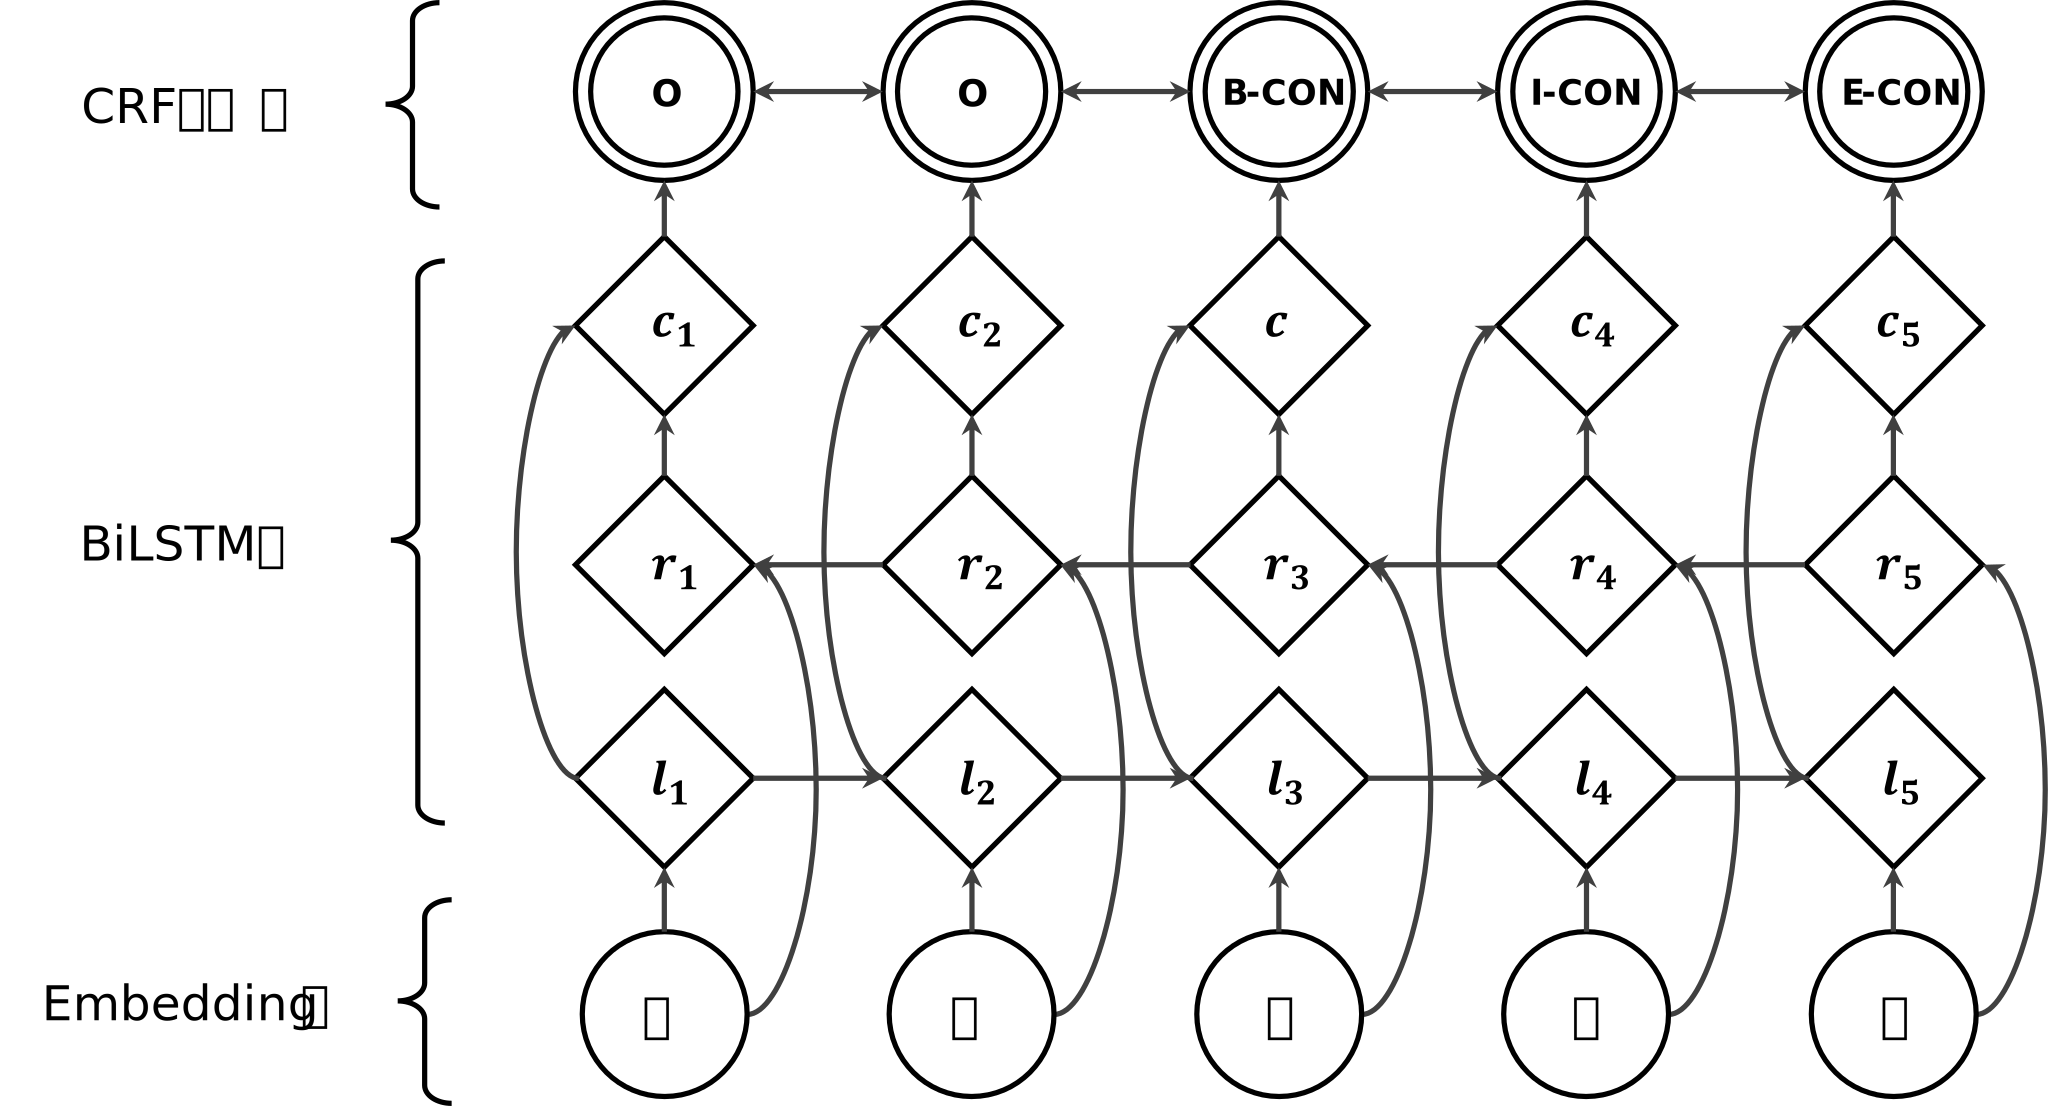
\includegraphics[width=0.85\linewidth]{ BiLSTM-CRF }
%	\caption{ 图片示例 }
%	\label{fig:BiLSTM-CRF}
%\end{figure}

\newpage

\section{作品测试与分析}

(建议包括测试方案、测试环境搭建、测试设备、测试数据、结果分析等)


\newpage

\section{创新性说明}

(本部分内容主要说明作品的创新性)

\newpage

\section{总结}

\newpage

%参考文献
\begin{thebibliography}{9}%宽度9
	\setlength{\itemsep}{-1mm}  %% 表示参考文献间距为行间距
	
	\bibitem{ref1}陈嘉莉,马自强,兰亚杰,等.基于区块链技术的医疗信息共享研究综述[J/OL].计算机应用研究:1-14[2024-05-12].https://doi.org/10.19734/j.issn.1001-3695.2023.12.0620.
	\bibitem{ref2}Bernd B .Authorisation and access control for electronic health record systems.[J].International journal of medical informatics,2004,73(3):251-7.
	\bibitem{ref3}Gustav J B ,Hoylen S ,Linda B , et al.Properties of a federated epidemiology query system.[J].International journal of medical informatics,2007,76(9):664-76.
	\bibitem{ref4}Nakamoto S.Bitcoin: A peer-to-peer electronic cash system[J]. Decentralized Business Review,2008: 21260.
	\bibitem{ref5}AZARIA A, EKBLAW A, VIEIRA T, et al. Medrec: Using blockchain for medical data access and permission management[C]//Proceedings of the 2016 2nd International Conference on Open and Big Data (OBD). Piscataway: IEEE, 2016: 25-30.
	\bibitem{ref6}Liu X, Hong Y, Sun J. Blockchain-based Medical Data Storage and Sharing System [C]// 2022 IEEE International Conference on Advances in Electrical Engineering and Computer Applications (AEECA) . IEEE, 2022: 62-66.
	\bibitem{ref7}尹嘉成. 基于区块链和IPFS的医疗数据共享模型[D].南京邮电大学,2022.DOI:10.27251/d.cnki.gnjdc.2021.000061.
	\bibitem{ref8}张悄. 基于联盟链的医疗数据多方共享系统设计与实现[D].北京邮电大学,2024.DOI:10.26969/d.cnki.gbydu.2023.002595.

\end{thebibliography}

\newpage
%附录
%\begin{appendices}
%
%\section{模板所用的宏包}
%\begin{table}[htbp]
%    \centering
%    \caption{宏包罗列}
%    \begin{tabular}{ccccc}
%        \toprule
%        \multicolumn{5}{c}{模板中已经加载的宏包} \\
%        \midrule
%        amsbsy & amsfonts & {amsgen} & {amsmath} & {amsopn} \\
%        amssymb & amstext & {appendix} & {array} & {atbegshi} \\
%        atveryend & auxhook & {bigdelim} & {bigintcalc} & {bigstrut} \\
%        bitset & bm    & {booktabs} & {calc} & {caption} \\
%        caption3 & CJKfntef & {cprotect} & {ctex} & {ctexhook} \\
%        ctexpatch & enumitem & {etexcmds} & {etoolbox} & {everysel} \\
%        expl3 & fix-cm & {fontenc} & {fontspec} & {fontspec-xetex} \\
%        geometry & gettitlestring & {graphics} & {graphicx} & {hobsub} \\
%        hobsub-generic & hobsub-hyperref & {hopatch} & {hxetex} & {hycolor} \\
%        hyperref & ifluatex & {ifpdf} & {ifthen} & {ifvtex} \\
%        ifxetex & indentfirst & {infwarerr} & {intcalc} & {keyval} \\
%        kvdefinekeys & kvoptions & {kvsetkeys} & {l3keys2e} & {letltxmacro} \\
%        listings & longtable & {lstmisc} & {ltcaption} & {ltxcmds} \\
%        multirow & nameref & {pdfescape} & {pdftexcmds} & {refcount} \\
%        rerunfilecheck & stringenc & {suffix} & {titletoc} & {tocloft} \\
%        trig  & ulem  & {uniquecounter} & {url} & {xcolor} \\
%        xcolor-patch & xeCJK & {xeCJKfntef} & {xeCJK-listings} & {xparse} \\
%        xtemplate & zhnumber &       &       &  \\
%        \bottomrule
%    \end{tabular}%
%    \label{tab:addlabel}%
%\end{table}%
%
%以上宏包都已经加载过了,不要重复加载它们。
%
%\section{排队算法--matlab 源程序}
%
%\begin{lstlisting}[language=matlab]
%kk=2;[mdd,ndd]=size(dd);
%while ~isempty(V)
%[tmpd,j]=min(W(i,V));tmpj=V(j);
%for k=2:ndd
%[tmp1,jj]=min(dd(1,k)+W(dd(2,k),V));
%tmp2=V(jj);tt(k-1,:)=[tmp1,tmp2,jj];
%end
%tmp=[tmpd,tmpj,j;tt];[tmp3,tmp4]=min(tmp(:,1));
%if tmp3==tmpd, ss(1:2,kk)=[i;tmp(tmp4,2)];
%else,tmp5=find(ss(:,tmp4)~=0);tmp6=length(tmp5);
%if dd(2,tmp4)==ss(tmp6,tmp4)
%ss(1:tmp6+1,kk)=[ss(tmp5,tmp4);tmp(tmp4,2)];
%else, ss(1:3,kk)=[i;dd(2,tmp4);tmp(tmp4,2)];
%end;end
%dd=[dd,[tmp3;tmp(tmp4,2)]];V(tmp(tmp4,3))=[];
%[mdd,ndd]=size(dd);kk=kk+1;
%end; S=ss; D=dd(1,:);
% \end{lstlisting}
%
% \section{规划解决程序--lingo源代码}
%
%\begin{lstlisting}[language=c]
%kk=2;
%[mdd,ndd]=size(dd);
%while ~isempty(V)
%    [tmpd,j]=min(W(i,V));tmpj=V(j);
%for k=2:ndd
%    [tmp1,jj]=min(dd(1,k)+W(dd(2,k),V));
%    tmp2=V(jj);tt(k-1,:)=[tmp1,tmp2,jj];
%end
%    tmp=[tmpd,tmpj,j;tt];[tmp3,tmp4]=min(tmp(:,1));
%if tmp3==tmpd, ss(1:2,kk)=[i;tmp(tmp4,2)];
%else,tmp5=find(ss(:,tmp4)~=0);tmp6=length(tmp5);
%if dd(2,tmp4)==ss(tmp6,tmp4)
%    ss(1:tmp6+1,kk)=[ss(tmp5,tmp4);tmp(tmp4,2)];
%else, ss(1:3,kk)=[i;dd(2,tmp4);tmp(tmp4,2)];
%end;
%end
%    dd=[dd,[tmp3;tmp(tmp4,2)]];V(tmp(tmp4,3))=[];
%    [mdd,ndd]=size(dd);
%    kk=kk+1;
%end;
%S=ss;
%D=dd(1,:);
% \end{lstlisting}
%\end{appendices}

%算法模板
%\begin{algorithm}[t]
%	\caption{algorithm caption} %算法的名字
%	\hspace*{0.02in} {\bf Input:} %算法的输入, \hspace*{0.02in}用来控制位置,同时利用 \\ 进行换行
%	input parameters A, B, C\\
%	\hspace*{0.02in} {\bf Output:} %算法的结果输出
%	output result
%	\begin{algorithmic}[1]
	%		\State some description % \State 后写一般语句
	%		\For{condition} % For 语句,需要和EndFor对应
	%		\If{condition} % If 语句,需要和EndIf对应
	%		\Else
	%		\EndIf
	%		\EndFor
	%		\While{condition} % While语句,需要和EndWhile对应
	%		a += 1
	%		\EndWhile
	%		\State\Return result
	%	\end{algorithmic}
%\end{algorithm}

%代码块模板
%\begin{lstlisting}[language=python]
%app_tuple_list = []
%try:
%browser.get(url)
%soup = BeautifulSoup(browser.page_source, features='lxml')
%except requests.HTTPError:
%return "There are some errors when get the download page!"
%all_app_tag = soup.find('ul', {"class": "applist", "id": "all-applist"})
%app_tag = all_app_tag.next
%\end{lstlisting}

\end{document} 